\begin{figure}[t]
\begin{center}
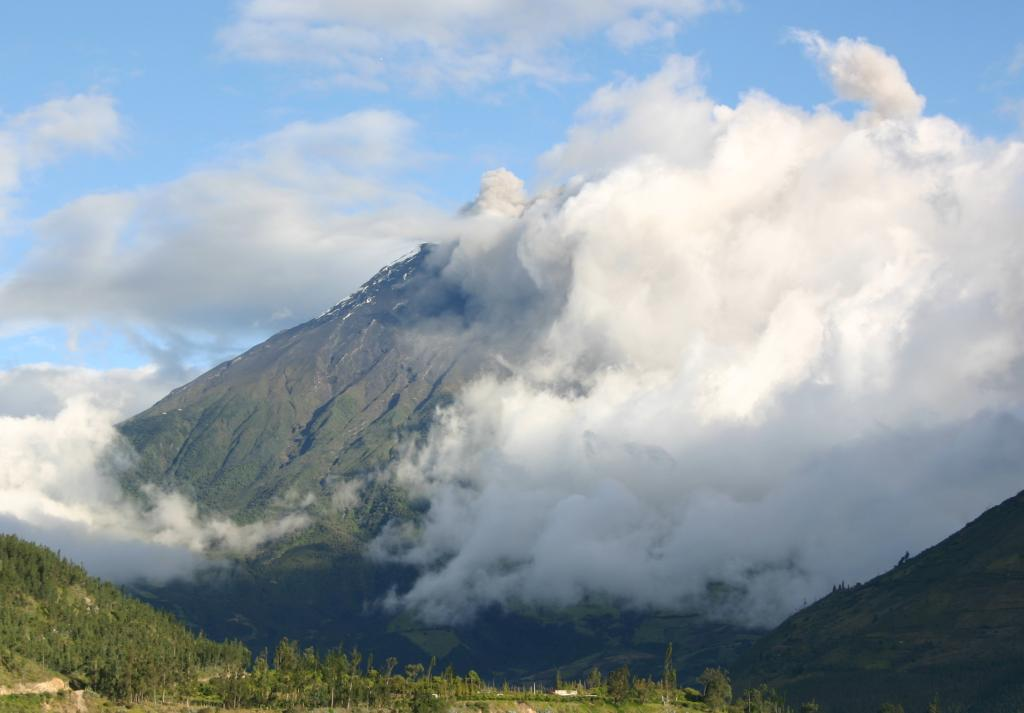
\includegraphics[width=0.9\hsize]{./figures/pics/tungurahua1.jpg}
\end{center}
\caption{\small {\bf Volc\'{a}n Tungurahua.}}
\label{fig-tungurahua}
\end{figure}

Volc\'{a}n Tungurahua (78.43$^\circ$W, 1.45$^\circ$S) is located on the
central part of the Eastern Cordillera of the Ecuadorean Andes
(Figures~\ref{fig-map}~and~\ref{fig-tungurahua}). Its current cone
has a steep flank (30-35$^\circ$ slopes) and a crater at the upper part of
its northwestern flank. Ba\~{n}os, an important tourist destination in
Ecuador with 25,000 inhabitants, is located at the foot of the volcano
close to Agoyan, one of the country's largest hydroelectric plants. Rural
communities are dispersed all around the volcano's lower flanks.

Geological studies show that Volc\'{a}n Tungurahua has produced Plinian-type
eruptions as well as at least two sector collapses ($\approx$ 13,000 
and 3,000 years b.p.~\cite{Hall99}). Since colonial times (1534), 
five eruptive cycles have occurred: 1641--1646, 1773--1781, 1886--1888,
1916--1918, and 1999--present. Generally, these eruptions were
characterized by tephra-and-ash falls covering the volcano flanks,
especially the western slopes, lahars, pyroclastic flows, and 
lava flows running down the north, west and south-western
valleys.

The current eruptive period was preceded by anomalous
seismicity first detected in 1993 by the local seismic
network~\cite{Ruiz94}.
In October 1999, after a few months of increasing
seismicity, Tungurahua emitted an ash column with incandescent blocks.
This activity led to the evacuation of more than 16,000 residents from
the surrounding areas.  As of August 2004, more than 1,900 volcanic
explosions have been recorded at Tungurahua by the Instituto Geof\'{i}sico
in Quito.  Activity has been grouped into eight eruptive cycles. The
last cycle started on May 2004 and reached its climax in June. These
eruptive periods have manifested ash emissions, and vulcanian and
strombolian activity. 

Volc\'{a}n Tungurahua is monitored by the Instituto Geof\'{i}sico of the
Escuela Politecnica Nacional (IGEPN) using a seismic network of seven
short-period stations, one broadband station, two tiltmeters, five
deformation
control lines, acoustic flow meters, and an SO$_2$-concentration
measurement system. In November 1999, a temporary microphone for
recording infrasound signals was deployed in a ridge just in front of
the volcano northwestern flank~\cite{Johnson03}.
In addition, numerous scientific campaigns, such as ours, have deployed 
temporary monitoring stations on the volcano.

